\section{Results}

\subsection{Datasets and Processing}
\label{data}
In our experiments, we have used whole genome sequencing data of two mother-father-child trios I1 (Table \ref{tab:I1}), and G1, published by \cite{kitzman2012}. In our experiments we have mainly used the first trio I1 with 13\% fetal admixture in obtained plasma. For maternal, paternal, and plasma datasets the reads were aligned to the hg19 genome using BWA. We genotyped both the parents using Samtools and Vcftools. To improve the precision of genotyping we only consider variants at positions previously identified as variable within the 1000 Genomes Project.  Subsequently we have phased the haplotypes using Beagle 4 \cite{browning2013} with reference haplotype panels from 1000 Genomes Project. 
\begin{table}[t]
\centering
\begin{tabular}{l|l|c}
Individual & Sample & DOC \\ \hline
Mother (I1-M) & Plasma (5 ml, gestational age 18.5 weeks) & 78 \\
	& Whole blood ($<1$ ml) & 32 \\
Father (I1-P) & Saliva & 39 \\
Child (I1-C) & Cord blood at delivery & 40
\end{tabular}
\vspace{3pt}
\caption{Summary of mother-father-child trio I1 sequencing data, curtsey of \cite{kitzman2012}  }
\label{tab:I1} 
\end{table}

\subsection{Evaluation}
\begin{table*}[t]
\centering
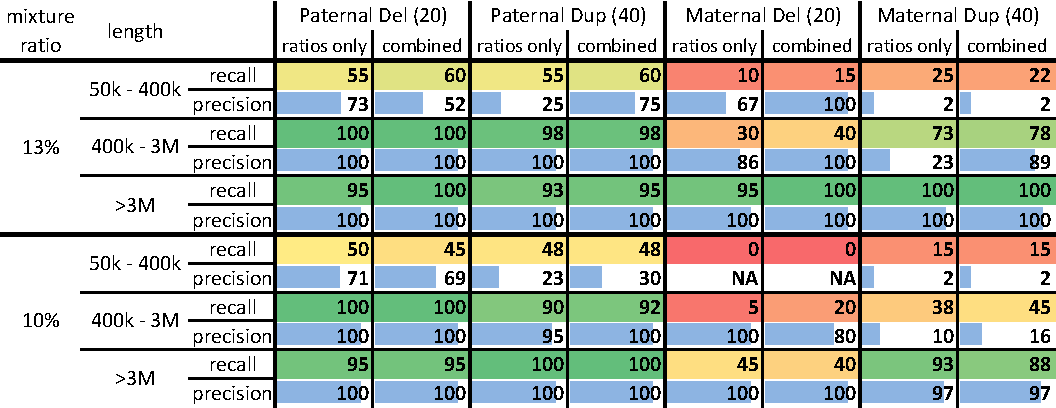
\includegraphics[width=0.85\textwidth]{figures/ismb_res_color}
%\vspace{3pt}
\caption{Summary of recall on test set composed of 360 \emph{in silico} simulated CNVs in I1 maternal plasma samples with 13\% and 10\% fetal admixture ratio. The ratios column corresponds to the method that only uses allelic ratios, but not the coverage prior. In such cases the precision is reduced, while the recall is largely unaffected.  }
\label{tab:resRecall} 
\end{table*}

We have simulated 360 CNVs in I1 plasma to test recall of our method, while G1 plasma sample served as a reference in DOC-based CNV estimation described in \ref{ss:coverage}. For each test case, we have picked a random position in chromosome 1, outside known centromere and telomeres regions, to place the simulated CNV.  We then ran our algorithm on a sequence window starting 20Mb before the simulated CNV and ending 20Mb after the CNV.  We describe our simulation methods in detail in the Section \ref{ss:simulation}. The results are shown in Table \ref{tab:resRecall}. We identify a CNV as identified if it is overlapped by CNVs of the same type by at least 50\%, while precision is computed as the fraction of correct CNVs over all identified of the current length in all experiments. To evaluate the effect the admixture has on accuracy, we repeated this experiment not only with the original plasma dataset, but also once down-sampled to only contain 10\% admixture. 

\begin{table*}[t]
\centering
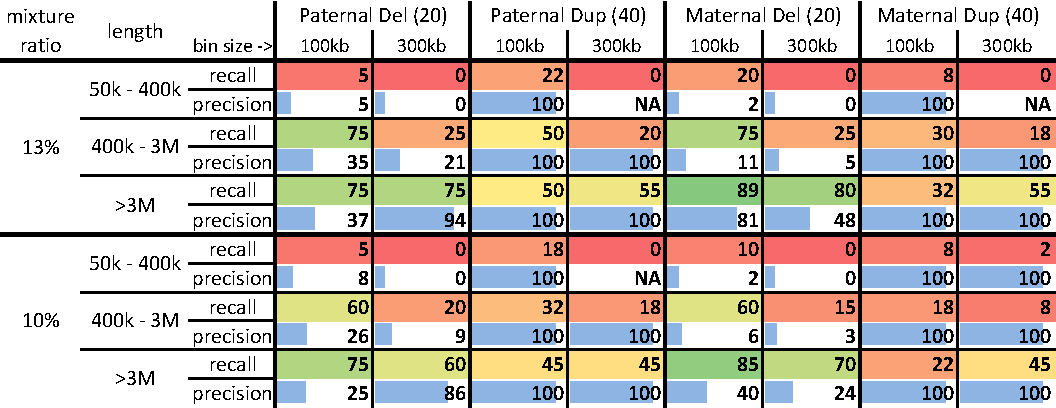
\includegraphics[width=0.85\textwidth]{figures/ismb_wrv_res_color}
\caption{Summary of results obtained by an HMM using only WRV signal. The same test set composed of 360 \emph{in silico} simulated CNVs was used as in Table \ref{tab:resRecall}. We performed the testing with 100kb and 300kb window sizes.}
\label{tab:resWRV} 
\end{table*}

The results indicate that our method can achieve nearly perfect recall and precision for variants $>3$ megabases, and promising results down to CNVs of 400 kilobases.  Maternally inherited events are typically more difficult to identify than paternally inherited ones, and deletions more difficult to duplications, possibly due to complete dropout of fetal alleles due to reduced admixture.

To test precision of our method, we run our model on the whole plasma dataset (expected to contain no large de-novo variants) and observed the number of CNV calls for each size. These numbers are shown in Table \ref{tab:resWGS}, with \textit{in silico} accuracy for each length shown for comparison. Notably, a large fraction of the larger false positive calls correspond to CNVs already present in parents (and hence inherited, rather than de novo). 

\begin{table*}
\centering
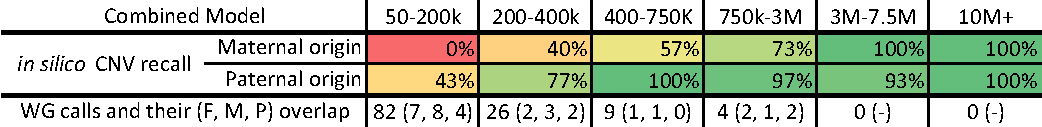
\includegraphics[width=0.78\textwidth]{figures/wg_calls_color}
\caption{In silico recall and number of CNVs of various sizes generated in a genome-wide run. For each CNV size we also show (in parenthesis) the number of calls that are from at least 50\% overlapped by CNVnator \cite{abyzov2011cnvnator} calls on the fetal, maternal, and paternal genomes, respectively.}
\label{tab:resWGS} 
\end{table*}
\vspace{1cm}

To implement our method we have used Python with PyPy interpreter. When run on chromosome 1 (the largest input size) our implementation required up to 18GB of RAM and took \ntilde 25 minutes of single thread CPU time to finish.
